% Created 2019-10-31 to 18:07
% Intended LaTeX compiler: pdflatex
\documentclass{article}

%%%% settings when exporting code %%%% 

\usepackage{listings}
\lstset{
backgroundcolor=\color{white},
basewidth={0.5em,0.4em},
basicstyle=\ttfamily\small,
breakatwhitespace=false,
breaklines=true,
columns=fullflexible,
commentstyle=\color[rgb]{0.5,0,0.5},
frame=single,
keepspaces=true,
keywordstyle=\color{black},
literate={~}{$\sim$}{1},
numbers=left,
numbersep=10pt,
numberstyle=\ttfamily\tiny\color{gray},
showspaces=false,
showstringspaces=false,
stepnumber=1,
stringstyle=\color[rgb]{0,.5,0},
tabsize=4,
xleftmargin=.23in,
emph={anova,apply,class,coef,colnames,colNames,colSums,dim,dcast,for,ggplot,head,if,ifelse,is.na,lapply,list.files,library,logLik,melt,plot,require,rowSums,sapply,setcolorder,setkey,str,summary,tapply},
emphstyle=\color{blue}
}

%%%% packages %%%%%

\usepackage[utf8]{inputenc}
\usepackage[T1]{fontenc}
\usepackage{lmodern}
\usepackage{textcomp}
\usepackage{color}
\usepackage{enumerate}
\usepackage{graphicx}
\usepackage{grffile}
\usepackage{wrapfig}
\usepackage{rotating}
\usepackage{longtable}
\usepackage{multirow}
\usepackage{multicol}
\usepackage{changes}
\usepackage{pdflscape}
\usepackage{geometry}
\usepackage[normalem]{ulem}
\usepackage{amssymb}
\usepackage{amsmath}
\usepackage{amsfonts}
\usepackage{dsfont}
\usepackage{array}
\usepackage{ifthen}
\usepackage{hyperref}
\usepackage{natbib}
\RequirePackage{fancyvrb}
\DefineVerbatimEnvironment{verbatim}{Verbatim}{fontsize=\small,formatcom = {\color[rgb]{0.5,0,0}}}
\RequirePackage{colortbl} % arrayrulecolor to mix colors
\RequirePackage{setspace} % to modify the space between lines - incompatible with footnote in beamer
\usepackage{authblk} % enable several affiliations (clash with beamer)
\renewcommand{\baselinestretch}{1.1}
\geometry{top=2cm}
\RequirePackage{epstopdf} % to be able to convert .eps to .pdf image files
\RequirePackage{capt-of}
\RequirePackage{caption}
\newcommand\model{\mathcal{M}}
\newcommand\Rlogo{\textbf{\textsf{R}}}
\RequirePackage{amsmath}
\RequirePackage{algorithm}
\RequirePackage[noend]{algpseudocode}
\RequirePackage{ifthen}
\RequirePackage{xspace} % space for newcommand macro
\RequirePackage{xifthen}
\RequirePackage{xargs}
\RequirePackage{dsfont}
\RequirePackage{amsmath,stmaryrd,graphicx}
\RequirePackage{prodint} % product integral symbol (\PRODI)
\RequirePackage{amsthm}
\newtheorem{theorem}{Theorem}
\newtheorem{lemma}[theorem]{Lemma}
\newcommand\defOperator[7]{%
\ifthenelse{\isempty{#2}}{
\ifthenelse{\isempty{#1}}{#7{#3}#4}{#7{#3}#4 \left#5 #1 \right#6}
}{
\ifthenelse{\isempty{#1}}{#7{#3}#4_{#2}}{#7{#3}#4_{#1}\left#5 #2 \right#6}
}
}
\newcommand\defUOperator[5]{%
\ifthenelse{\isempty{#1}}{
#5\left#3 #2 \right#4
}{
\ifthenelse{\isempty{#2}}{\underset{#1}{\operatornamewithlimits{#5}}}{
\underset{#1}{\operatornamewithlimits{#5}}\left#3 #2 \right#4}
}
}
\newcommand{\defBoldVar}[2]{
\ifthenelse{\equal{#2}{T}}{\boldsymbol{#1}}{\mathbf{#1}}
}
\newcommandx\Cov[2][1=,2=]{\defOperator{#1}{#2}{C}{ov}{\lbrack}{\rbrack}{\mathbb}}
\newcommandx\Esp[2][1=,2=]{\defOperator{#1}{#2}{E}{}{\lbrack}{\rbrack}{\mathbb}}
\newcommandx\Prob[2][1=,2=]{\defOperator{#1}{#2}{P}{}{\lbrack}{\rbrack}{\mathbb}}
\newcommandx\Qrob[2][1=,2=]{\defOperator{#1}{#2}{Q}{}{\lbrack}{\rbrack}{\mathbb}}
\newcommandx\Var[2][1=,2=]{\defOperator{#1}{#2}{V}{ar}{\lbrack}{\rbrack}{\mathbb}}
\newcommandx\Binom[2][1=,2=]{\defOperator{#1}{#2}{B}{}{(}{)}{\mathcal}}
\newcommandx\Gaus[2][1=,2=]{\defOperator{#1}{#2}{N}{}{(}{)}{\mathcal}}
\newcommandx\Wishart[2][1=,2=]{\defOperator{#1}{#2}{W}{ishart}{(}{)}{\mathcal}}
\newcommandx\Likelihood[2][1=,2=]{\defOperator{#1}{#2}{L}{}{(}{)}{\mathcal}}
\newcommandx\Information[2][1=,2=]{\defOperator{#1}{#2}{I}{}{(}{)}{\mathcal}}
\newcommandx\Score[2][1=,2=]{\defOperator{#1}{#2}{S}{}{(}{)}{\mathcal}}
\newcommandx\Vois[2][1=,2=]{\defOperator{#1}{#2}{V}{}{(}{)}{\mathcal}}
\newcommandx\IF[2][1=,2=]{\defOperator{#1}{#2}{IF}{}{(}{)}{\mathcal}}
\newcommandx\Ind[1][1=]{\defOperator{}{#1}{1}{}{(}{)}{\mathds}}
\newcommandx\Max[2][1=,2=]{\defUOperator{#1}{#2}{(}{)}{min}}
\newcommandx\Min[2][1=,2=]{\defUOperator{#1}{#2}{(}{)}{max}}
\newcommandx\argMax[2][1=,2=]{\defUOperator{#1}{#2}{(}{)}{argmax}}
\newcommandx\argMin[2][1=,2=]{\defUOperator{#1}{#2}{(}{)}{argmin}}
\newcommandx\cvD[2][1=D,2=n \rightarrow \infty]{\xrightarrow[#2]{#1}}
\newcommandx\Hypothesis[2][1=,2=]{
\ifthenelse{\isempty{#1}}{
\mathcal{H}
}{
\ifthenelse{\isempty{#2}}{
\mathcal{H}_{#1}
}{
\mathcal{H}^{(#2)}_{#1}
}
}
}
\newcommandx\dpartial[4][1=,2=,3=,4=\partial]{
\ifthenelse{\isempty{#3}}{
\frac{#4 #1}{#4 #2}
}{
\left.\frac{#4 #1}{#4 #2}\right\rvert_{#3}
}
}
\newcommandx\dTpartial[3][1=,2=,3=]{\dpartial[#1][#2][#3][d]}
\newcommandx\ddpartial[3][1=,2=,3=]{
\ifthenelse{\isempty{#3}}{
\frac{\partial^{2} #1}{\left( \partial #2\right)^2}
}{
\frac{\partial^2 #1}{\partial #2\partial #3}
}
}
\newcommand\Real{\mathbb{R}}
\newcommand\Rational{\mathbb{Q}}
\newcommand\Natural{\mathbb{N}}
\newcommand\trans[1]{{#1}^\intercal}%\newcommand\trans[1]{{\vphantom{#1}}^\top{#1}}
\newcommand{\independent}{\mathrel{\text{\scalebox{1.5}{$\perp\mkern-10mu\perp$}}}}
\newcommand\half{\frac{1}{2}}
\newcommand\normMax[1]{\left|\left|#1\right|\right|_{max}}
\newcommand\normTwo[1]{\left|\left|#1\right|\right|_{2}}
\author{Brice Ozenne}
\date{\today}
\title{Assessing the effect of an exposure on multiple outcomes (with \Rlogo{} code)}
\hypersetup{
 colorlinks=true,
 citecolor=[rgb]{0,0.5,0},
 urlcolor=[rgb]{0,0,0.5},
 linkcolor=[rgb]{0,0,0.5},
 pdfauthor={Brice Ozenne},
 pdftitle={Assessing the effect of an exposure on multiple outcomes (with \Rlogo{} code)},
 pdfkeywords={},
 pdfsubject={},
 pdfcreator={Emacs 25.2.1 (Org mode 9.0.4)},
 pdflang={English}
 }
\begin{document}

\maketitle

\section*{Summary}
\label{sec:orgb4c3585}
We propose a strategy to assess the effect of an exposure (e.g. a
disease, a genetic factor) on several outcomes (e.g. psychological
outcomes, the binding potential measured in several brain regions)
while accounting for possible risk factors and confounders. This
strategy, called \emph{multiple univariage regressions} strategy, models
the relationship between each outcome and the exposure using a
separate model. Once the models have been correctly fitted, a global
test can be used to test whether there is any effect of the exposure
on the outcomes. After that, multiple tests are performed to test
outcome-specific effects of the exposure where the Dunnett adjustment
is used to control the type 1 error \citep{pipper2012versatile}. An
adjustment is used to improved the control of the type 1 error in
small sample sizes (e.g. n<100). This adjustment has been shown to
beneficial in several settings (using simulation studies) but does not
always perfectly control the type 1 error rate. It is advised to check
that validity of the adjustment when using very small samples or
models with many parameters.

\bigskip

The proposed strategy can be used with any type of outcomes for which
  a can fit a model with asymptotically linear estimators
  (\cite{tsiatis2007semiparametric}, section 3). This includes
  generalized linear model or Cox models. It makes it very flexible
  and the strategy makes only few assumptions on the joint
  distribution. The drawback is that it is not the most efficient
  approach. For instance modelling the joint distribution of the
  outcomes, e.g. using a latent variable model / mixed model in the
  case of normally distributed outcomes, will be a more efficient
  strategy. Another limitation is that with the proposed approach a
  treatment effect specific to each outcome will be estimated, while
  in some context the investigator may want to constrain the treatment
  effect to be the same for some outcomes. Finally, to be feasible the
  strategy requires the number of outcomes to be not too large (<100)
  and smaller than the number of observations (low-dimensional
  setting).

\bigskip

This document we aim at giving a basic understanding of the strategy
  and how to implement it. In particular, we don't claim that the
  proposed strategy is valid or optimal results in every application
  (it is probably not the case) and many other approaches exists but
  won't be discussed here. The document is organized as follow: first
  section \ref{sec:Rsoftware} present how to install and set up the
  \Rlogo{} software. Then basic functions to import and process the
  data are presented in section \ref{sec:dataManagement}. The goals, a
  minima, of the descriptive analysis are presented in section
  \ref{sec:descriptive}, as well as code to export figures and tables to
  Word documents. Section \ref{sec:LM} recalls how to perform a univariate
  linear regression in \Rlogo{} and present tools to assess the
  parametric assumptions and section \ref{sec:multipleLM} presents the
  \emph{multiple univariate regressions} strategy. Finally appendix
  \ref{SM:statistics} recalls some statistical concepts about modeling and
  hypothesis testing.

\clearpage

\section{Software}
\label{sec:Rsoftware}
We advise to use the \Rlogo{} software to implement these strategies. It can
be downloaded at \url{https://cloud.r-project.org/}. R studio provide a
convenient user interface that can be downloaded at
\url{https://www.rstudio.com/products/rstudio/}.  The \Rlogo{} code used to carry
out the two strategies will be display in boxes:
\lstset{language=r,label= ,caption= ,captionpos=b,numbers=none}
\begin{lstlisting}
1+1 ## comment about the code
\end{lstlisting}

\begin{verbatim}
[1] 2
\end{verbatim}

while the \Rlogo{} output will be displayed in dark red below the box. 

\bigskip

When starting a fresh \Rlogo{} session, only the core functionalities of
\Rlogo{} are available. Additional functionalities called packages can
be downloaded from the CRAN using the command \texttt{install.packages}. We
will need the following packages:
\lstset{language=r,label= ,caption= ,captionpos=b,numbers=none}
\begin{lstlisting}
install.packages(pkgs = c("lava","lavaSearch2","multcomp","qqtest","gof","reshape2"))
\end{lstlisting}

After having installed the packages, one needs to load them using the
command \texttt{library} to use them in the current \Rlogo{} session:
\lstset{language=r,label= ,caption= ,captionpos=b,numbers=none}
\begin{lstlisting}
library(lava) ## definition and estimation of latent variable models
library(lavaSearch2) ## small sample correction 
library(multcomp) ## adjustment for multiple comparisons
library(qqtest) ## diagnostics: qqplots
library(gof) ## diagnostics: linearity assumption
library(reshape2) ## data management
\end{lstlisting}

I also recommend the following packages:
\begin{itemize}
\item \emph{data.table}: for data management. See
\url{https://cran.r-project.org/web/packages/data.table/vignettes/datatable-intro.html}
for an introduction and
\url{https://github.com/Rdatatable/data.table/wiki} for more
documentation.  A synthetic description of the functionalities can
be found at
\url{https://s3.amazonaws.com/assets.datacamp.com/img/blog/data+table+cheat+sheet.pdf}
\item \emph{ggplot2}: for data visualization. See
\url{http://r4ds.had.co.nz/data-visualisation.html} for an introduction. A
synthetic description of the functionalities can be found at
\url{https://www.rstudio.com/wp-content/uploads/2015/03/ggplot2-cheatsheet.pdf}
\end{itemize}

\clearpage

\section{Data management}
\label{sec:dataManagement}
\subsection{Working directory}
\label{sec:org47efbee}

The working directory is where R, by default, look for files
to import and export data or figures. The current working directory
can be accessed using:
\lstset{language=r,label= ,caption= ,captionpos=b,numbers=none}
\begin{lstlisting}
getwd()
\end{lstlisting}

\begin{verbatim}
[1] "c:/Users/hpl802/AppData/Roaming/R"
\end{verbatim}

It can be changed using the function \texttt{setwd()}:
\lstset{language=r,label= ,caption= ,captionpos=b,numbers=none}
\begin{lstlisting}
path <- "c:/"
setwd(path)
\end{lstlisting}

We can check that the working directory has indeed changed calling
again \texttt{getwd()}:
\lstset{language=r,label= ,caption= ,captionpos=b,numbers=none}
\begin{lstlisting}
getwd()
\end{lstlisting}

\begin{verbatim}
[1] "c:/"
\end{verbatim}

\subsection{Importing the data}
\label{sec:org63acd04}

It is a good idea to start by checking that the working directory
contains the data we want to import. For instance the file \texttt{data.csv}
is storing the data, we can use:
\lstset{language=r,label= ,caption= ,captionpos=b,numbers=none}
\begin{lstlisting}
file.exists("data.csv")
\end{lstlisting}

\begin{verbatim}
[1] TRUE
\end{verbatim}

We can also list all files in the current directory with a \texttt{.csv} extension using:
\lstset{language=r,label= ,caption= ,captionpos=b,numbers=none}
\begin{lstlisting}
list.files(pattern = ".csv")
\end{lstlisting}

\begin{verbatim}
[1] "data.csv"
\end{verbatim}

We can also display the first lines of the file using:
\lstset{language=r,label= ,caption= ,captionpos=b,numbers=none}
\begin{lstlisting}
readLines("data.csv")[1:3]
\end{lstlisting}

\begin{verbatim}
[1] "\"Id\",\"Gender\",\"age\",\"BMI\",\"MDI\",\"Y1\",\"Y2\",\"Y3\",\"Y4\",\"Y5\""
[2] "\"Subj1\",\"female\",30.57,21.76,25.82,7.64,8.73,7.72,10.42,8.44"            
[3] "\"Subj2\",\"female\",41.36,25.55,12.38,7.11,8.79,6.99,8.45,8.26"
\end{verbatim}

We can see that the columns are separated with \texttt{,} and that the \texttt{.}
indicates the decimal values. Moreover the words such as the columns
names or the subject identities are surrounded by \texttt{\textbackslash{}"} (e.g. \texttt{\textbackslash{}"Id\textbackslash{}"}
stand for Id). Finally in this example there is no missing values but
if there was it is important to know how they are encoded.

\clearpage

 The command to import the data depends on the type of file. Here for
a \texttt{.csv} file we use \texttt{read.csv}. Luckily the default arguments \texttt{sep},
\texttt{dec}, \texttt{quote} are correctly specified:
\lstset{language=r,label= ,caption= ,captionpos=b,numbers=none}
\begin{lstlisting}
args(read.csv)
\end{lstlisting}

\begin{verbatim}
function (file, header = TRUE, sep = ",", quote = "\"", dec = ".", 
    fill = TRUE, comment.char = "", ...) 
NULL
\end{verbatim}

The argument \texttt{header} set to \texttt{TRUE} indicates that the first line of
the dataset contains the column names (and not the actual data). The
\texttt{...} indicates there are additional arguments that are not shown here
(see the documentation using \texttt{help(read.csv)}). For instance, in
presence of missing values, one would need to specify the argument
\texttt{na.string}. Here it is sufficient to do:
\lstset{language=r,label= ,caption= ,captionpos=b,numbers=none}
\begin{lstlisting}
dfW <- read.csv("data.csv")
\end{lstlisting}

Other functions exists to import other types of data,
e.g. \texttt{read.table} for \texttt{.txt} files, \texttt{read.xlsx} from the xlsx package
for \texttt{.xlsx} file, or \texttt{read.spss} from the foreign package for spss
data files. One should always inspect if R has correctly imported the
data, e.g. using:
\lstset{language=r,label= ,caption= ,captionpos=b,numbers=none}
\begin{lstlisting}
str(dfW)
\end{lstlisting}

\begin{verbatim}
'data.frame':	50 obs. of  10 variables:
 $ Id    : Factor w/ 50 levels "Subj1","Subj10",..: 1 12 23 34 45 47 48 49 50 2 ...
 $ Gender: Factor w/ 2 levels "female","male": 1 1 2 1 1 1 2 1 2 2 ...
 $ age   : num  30.6 41.4 27 40.6 45.8 ...
 $ BMI   : num  21.8 25.6 28.6 23.2 19.8 ...
 $ MDI   : num  25.82 12.38 7.41 16.46 18.56 ...
 $ Y1    : num  7.64 7.11 7.88 8.99 7.6 6.99 3.76 6.94 6.57 6.89 ...
 $ Y2    : num  8.73 8.79 9.89 14.38 8.77 ...
 $ Y3    : num  7.72 6.99 13.51 13.82 8.38 ...
 $ Y4    : num  10.42 8.45 10.79 11.44 7.94 ...
 $ Y5    : num  8.44 8.26 7.9 9.75 6.17 8.78 2.41 5.38 5.04 5.22 ...
\end{verbatim}

In this example, the two columns contain character strings (\texttt{Factor}
is a type of character strings in R) and the rest contains numerical
values.

\subsection{Data processing}
\label{sec:orgf47fb73}

Often the raw data needs to be transformed before being analyzed:
\begin{itemize}
\item A typical example is when one need to deal with the variable:
\end{itemize}
\lstset{language=r,label= ,caption= ,captionpos=b,numbers=none}
\begin{lstlisting}
gender <- c(1,0,1,0,1) ## what is 1? what is 0?
\end{lstlisting}

This is already better:
\lstset{language=r,label= ,caption= ,captionpos=b,numbers=none}
\begin{lstlisting}
female <- c(1,0,1,0,1) ## we can guess that 1: female and 0: male
\end{lstlisting}

\clearpage 

but it is a good practice in such situation to rename the actual
values into something understandable:
\lstset{language=r,label= ,caption= ,captionpos=b,numbers=none}
\begin{lstlisting}
factor(gender, levels = 0:1, labels = c("Female","Male"))
\end{lstlisting}

\begin{verbatim}
[1] Male   Female Male   Female Male  
Levels: Female Male
\end{verbatim}

\begin{itemize}
\item With repeated measurements per individual, one often needs to
reshape his dataset from the wide format (one line per individual)
to the long format (one line per measurement). This can be done
using the \texttt{melt} method:
\end{itemize}
\lstset{language=r,label= ,caption= ,captionpos=b,numbers=none}
\begin{lstlisting}
dfL <- melt(dfW, 
			id.vars = c("Id","Gender","age","BMI","MDI"),
			value.name = "score",
			variable.name = "outcome")
head(dfL)
\end{lstlisting}

\begin{verbatim}
     Id Gender   age   BMI   MDI outcome score
1 Subj1 female 30.57 21.76 25.82      Y1  7.64
2 Subj2 female 41.36 25.55 12.38      Y1  7.11
3 Subj3   male 26.97 28.56  7.41      Y1  7.88
4 Subj4 female 40.61 23.22 16.46      Y1  8.99
5 Subj5 female 45.79 19.78 18.56      Y1  7.60
6 Subj6 female 37.14 16.13 17.82      Y1  6.99
\end{verbatim}

The opposite operation can be performed using \texttt{dcast}.

\begin{itemize}
\item It is often a good idea to restrict the dataset to the relevant
variables (e.g. remove genetic data if they are not of interest). It
is easier to work with and to display in the next steps. This can
for instance be done by defining the variables of interest:
\end{itemize}
\lstset{language=r,label= ,caption= ,captionpos=b,numbers=none}
\begin{lstlisting}
keep.var <- c("Id","BMI","MDI","Y1","Y2","Y3","Y4","Y5")
\end{lstlisting}

We can check that the variables defined in \texttt{keep.var} are in \texttt{dfW}:
\lstset{language=r,label= ,caption= ,captionpos=b,numbers=none}
\begin{lstlisting}
keep.var %in% names(dfW)
\end{lstlisting}

\begin{verbatim}
[1] TRUE TRUE TRUE TRUE TRUE TRUE TRUE TRUE
\end{verbatim}

and then subset the initial dataset:
\lstset{language=r,label= ,caption= ,captionpos=b,numbers=none}
\begin{lstlisting}
dfW.red <- dfW[,keep.var]
head(dfW.red)
\end{lstlisting}

\begin{verbatim}
     Id   BMI   MDI   Y1    Y2    Y3    Y4   Y5
1 Subj1 21.76 25.82 7.64  8.73  7.72 10.42 8.44
2 Subj2 25.55 12.38 7.11  8.79  6.99  8.45 8.26
3 Subj3 28.56  7.41 7.88  9.89 13.51 10.79 7.90
4 Subj4 23.22 16.46 8.99 14.38 13.82 11.44 9.75
5 Subj5 19.78 18.56 7.60  8.77  8.38  7.94 6.17
6 Subj6 16.13 17.82 6.99  9.97  6.74  8.29 8.78
\end{verbatim}

\begin{itemize}
\item Often after having imported the data we want to change its column
names. First we need to know the current column names. The \texttt{names}
function can be used to output all the column names:
\end{itemize}
\lstset{language=r,label= ,caption= ,captionpos=b,numbers=none}
\begin{lstlisting}
names(dfW.red)
\end{lstlisting}

\begin{verbatim}
[1] "Id"  "BMI" "MDI" "Y1"  "Y2"  "Y3"  "Y4"  "Y5"
\end{verbatim}

Alternatively the \texttt{grep} function will output any column name
containing a given string of characters:
\lstset{language=r,label= ,caption= ,captionpos=b,numbers=none}
\begin{lstlisting}
grep(pattern = "Y", x = names(dfW), value = TRUE)
\end{lstlisting}

\begin{verbatim}
[1] "Y1" "Y2" "Y3" "Y4" "Y5"
\end{verbatim}

Then, we can rename a specific column using:
\lstset{language=r,label= ,caption= ,captionpos=b,numbers=none}
\begin{lstlisting}
names(dfW.red)[names(dfW.red) == "Id"] <- "new.Id.name"
head(dfW.red)
\end{lstlisting}

\begin{verbatim}
  new.Id.name   BMI   MDI   Y1    Y2    Y3    Y4   Y5
1       Subj1 21.76 25.82 7.64  8.73  7.72 10.42 8.44
2       Subj2 25.55 12.38 7.11  8.79  6.99  8.45 8.26
3       Subj3 28.56  7.41 7.88  9.89 13.51 10.79 7.90
4       Subj4 23.22 16.46 8.99 14.38 13.82 11.44 9.75
5       Subj5 19.78 18.56 7.60  8.77  8.38  7.94 6.17
6       Subj6 16.13 17.82 6.99  9.97  6.74  8.29 8.78
\end{verbatim}

To rename several columns at the same time we can use:
\lstset{language=r,label= ,caption= ,captionpos=b,numbers=none}
\begin{lstlisting}
old2new <- c("Y1" = "y1", "Y2" = "y2", "Y3" = "y3")
names(dfW.red)[match(names(old2new),names(dfW.red))] <- old2new
head(dfW.red)
\end{lstlisting}

\begin{verbatim}
  new.Id.name   BMI   MDI   y1    y2    y3    Y4   Y5
1       Subj1 21.76 25.82 7.64  8.73  7.72 10.42 8.44
2       Subj2 25.55 12.38 7.11  8.79  6.99  8.45 8.26
3       Subj3 28.56  7.41 7.88  9.89 13.51 10.79 7.90
4       Subj4 23.22 16.46 8.99 14.38 13.82 11.44 9.75
5       Subj5 19.78 18.56 7.60  8.77  8.38  7.94 6.17
6       Subj6 16.13 17.82 6.99  9.97  6.74  8.29 8.78
\end{verbatim}

Other useful functions are \texttt{tolower} to convert characters to lower
case and \texttt{gsub} to remove a specific pattern in a character vector, e.g.:
\lstset{language=r,label= ,caption= ,captionpos=b,numbers=none}
\begin{lstlisting}
gsub(pattern = ".", replacement = "", x = c("a..","b..."), fixed = TRUE)
\end{lstlisting}

\begin{verbatim}
[1] "a" "b"
\end{verbatim}

Many of the other data processing steps are specific to each study and
we won't discuss them in this document. 

\clearpage

\section{Descriptive statistics}
\label{sec:descriptive}
Before doing any analysis, it is a good practice to describe the data
that are to be analyzed. The has several aims:
\begin{itemize}
\item \textbf{check that that database contains the population of interest},
i.e. individuals in the database are indeed those the we want to
study and we have all of them.
\item \textbf{check that the collected values are plausible}, e.g. if the inclusion
criteria include that the age range is between 18 and 99 years, then
one should check that this is indeed the case.
\item \textbf{check that the collected values are coded as expected}, e.g. age is
usually coded in years (and not in months).
\item \textbf{check that the collected values are distributed as expected},
e.g. is there missing values? Are the values uniformly spread?
Bimodal? Concentrated at low or high values?
\end{itemize}

Note: one should checks that for all the variables of interest. This
can appear time-consuming but can really save you time at latter
stages. 

\begin{itemize}
\item \textbf{produce your table 1} i.e. a descriptive table of your cohort that
is almost always included in an article. You can for instance use
the function \texttt{univariateTable} from the Publish package:
\end{itemize}
\lstset{language=r,label= ,caption= ,captionpos=b,numbers=none}
\begin{lstlisting}
library(Publish)
myTable1 <- univariateTable(Gender ~ age + BMI + MDI + Y1 + Y2 + Y3 + Y4 + Y5, 
							data = dfW)
myTable1
\end{lstlisting}

\begin{verbatim}
  Variable     Level female (n=30) male (n=20) Total (n=50) p-value
1      age mean (sd)    36.2 (5.8)  34.6 (5.0)   35.6 (5.5) 0.31204
2      BMI mean (sd)    21.5 (3.3)  23.1 (3.2)   22.2 (3.4) 0.09325
3      MDI mean (sd)    19.2 (5.8)  19.2 (5.7)   19.2 (5.7) 0.97596
4       Y1 mean (sd)     7.2 (1.6)   7.2 (2.0)    7.2 (1.8) 0.93155
5       Y2 mean (sd)     9.6 (2.9)   9.5 (2.1)    9.6 (2.6) 0.82411
6       Y3 mean (sd)     8.5 (3.4)   8.4 (3.2)    8.4 (3.3) 0.91260
7       Y4 mean (sd)     8.8 (2.1)   9.3 (1.7)    9.0 (1.9) 0.39083
8       Y5 mean (sd)     7.4 (2.9)   7.0 (2.9)    7.2 (2.9) 0.65171
\end{verbatim}

You can also export this table in a word document with the package
officer:
\lstset{language=r,label= ,caption= ,captionpos=b,numbers=none}
\begin{lstlisting}
library(officer)
myTable1.doc <- body_add_table(x = read_docx(), 
							   value =  summary(myTable1)) 
print(myTable1.doc, target = "./Table1.docx")
\end{lstlisting}

To keep the code simple, we only present here a very basic application
of these tools. More complex tables with a nicer display in word can
be obtain with a bit of coding.

\clearpage

\begin{itemize}
\item \textbf{make synthetic representations of your data} using graphs or
images. This can be useful to visualize your data and help your
collaborators to understand what you have collected or what you are
trying to show.
\end{itemize}

\lstset{language=r,label= ,caption= ,captionpos=b,numbers=none}
\begin{lstlisting}
library(ggplot2)
gg <- ggplot(dfL, aes(x = MDI, y = score, color = Gender, group = Gender))
gg <- gg + geom_point()
gg <- gg + facet_wrap(~outcome, labeller = label_both)
gg <- gg + geom_smooth(method = "lm", se = FALSE)
gg
\end{lstlisting}

\begin{center}
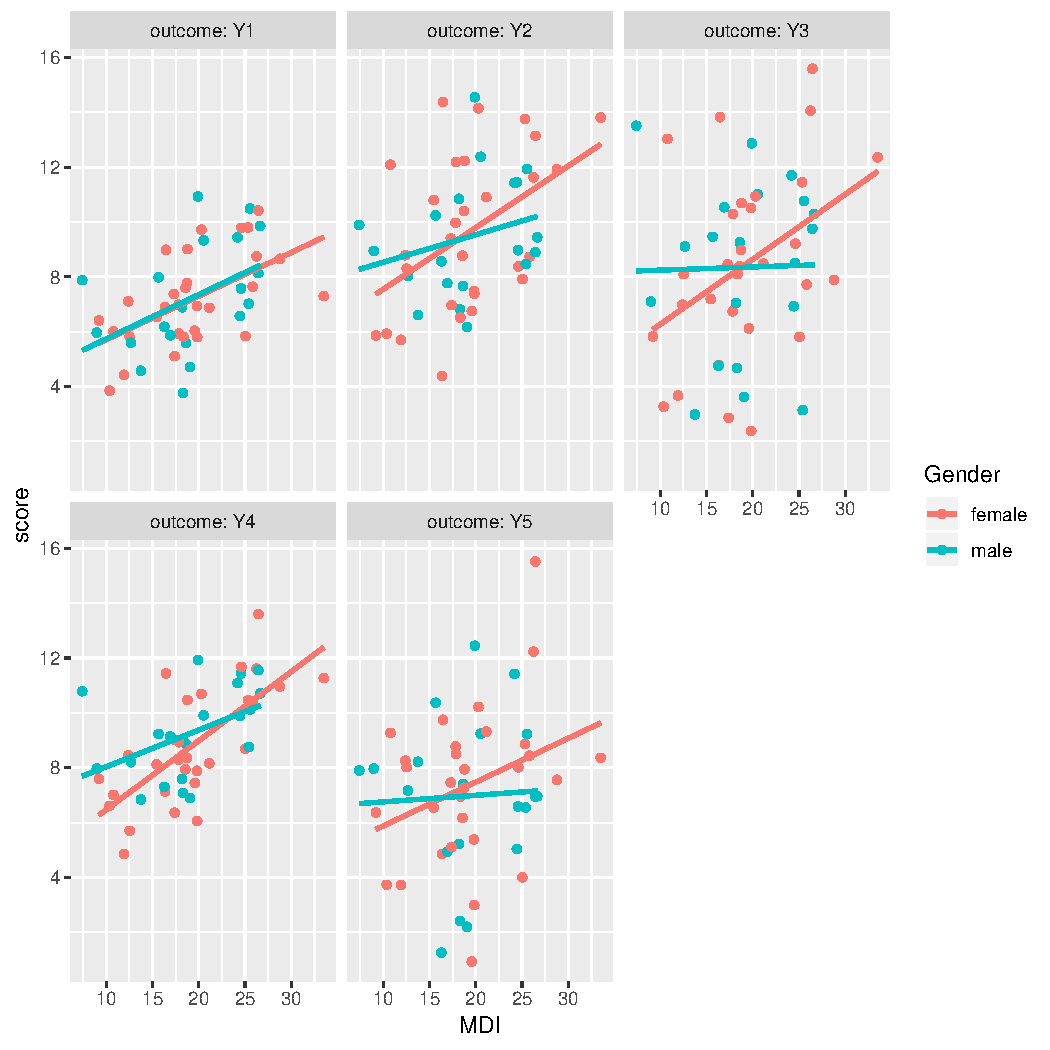
\includegraphics[width=.9\linewidth]{./figures/descriptive.pdf}
\end{center}

You can then export the figure using:
\lstset{language=r,label= ,caption= ,captionpos=b,numbers=none}
\begin{lstlisting}
pdf("./figures/descriptive.pdf")
gg
dev.off()
\end{lstlisting}

\begin{itemize}
\item \textbf{Compare percentages when considering categorical data}: the usual
way to compare the distribution of a categorical variable between
two groups is to run a Fisher test using \texttt{fisher.test} in the R
software. It returns a p-value and an estimate of the odd ratio with
its confidence interval. For instance, consider the following
dataset:
\end{itemize}
\lstset{language=r,label= ,caption= ,captionpos=b,numbers=none}
\begin{lstlisting}
mytable <- rbind(c(8,5),
				 c(4,15))
dimnames(mytable) <- list(c("control","treatment"),
						  c("-","+"))
mytable
\end{lstlisting}

\begin{verbatim}
          -  +
control   8  5
treatment 4 15
\end{verbatim}
The Fisher test outputs:
\lstset{language=r,label= ,caption= ,captionpos=b,numbers=none}
\begin{lstlisting}
fisher.test(mytable)
\end{lstlisting}

\begin{verbatim}
	Fisher's Exact Test for Count Data

data:  mytable
p-value = 0.02996
alternative hypothesis: true odds ratio is not equal to 1
95 percent confidence interval:
  0.9953576 38.7853302
sample estimates:
odds ratio 
  5.622612
\end{verbatim}

This approach admits two drawbacks:
\begin{itemize}
\item the p-value may not agree with the confidence interval of the odd
ratio regarding the rejection of the null hypothesis
\item the odd ratio is a rather complex quantity to understand.
\end{itemize}
Instead one can use the function \texttt{binomMeld.test} (package \emph{exact2x2})
to perform a test on the proportions:
\lstset{language=r,label= ,caption= ,captionpos=b,numbers=none}
\begin{lstlisting}
binomMeld.test(x1=mytable["control","+"],n1=sum(mytable["control",]),
			   x2=mytable["treatment","+"],n2=sum(mytable["treatment",]),
			   parmtype="difference")
\end{lstlisting}

\begin{verbatim}
	melded binomial test for difference

data:  sample 1:(5/13), sample 2:(15/19)
proportion 1 = 0.38462, proportion 2 = 0.78947, p-value = 0.05077
alternative hypothesis: true difference is not equal to 0
95 percent confidence interval:
 -0.001077177  0.715576028
sample estimates:
difference (p2-p1) 
         0.4048583
\end{verbatim}

This time the p-value is consistent with the confidence interval. In
fact, the p-value is matches the p-value of the confidence interval of
\texttt{fisher.test}:
\lstset{language=r,label= ,caption= ,captionpos=b,numbers=none}
\begin{lstlisting}
exact2x2(mytable, tsmethod = "central")
\end{lstlisting}

\begin{verbatim}
	Central Fisher's Exact Test

data:  mytable
p-value = 0.05077
alternative hypothesis: true odds ratio is not equal to 1
95 percent confidence interval:
  0.9953576 38.7853302
sample estimates:
odds ratio 
  5.622612
\end{verbatim}

The appropriate reference for this approach is \citep{fay2015combining}.
\clearpage

\section{Univariate analysis using a univariate linear regression}
\label{sec:LM}
Imagine we want to assess the effect of MDI on \(Y_1\)
adjusting for age and BMI using a univariate linear
regression. Mathematically the model can be written:
\begin{align}
Y_1 = \alpha + \beta_{age} age + \beta_{BMI} BMI + \beta_{MDI} MDI + \varepsilon \label{eq:lm}
\end{align}
where \(\varepsilon\) are the residuals. that are assumed to be:
\begin{itemize}
\item A0: independent and identically distributed (iid)
\item A1: normally distributed.
\end{itemize}
Note that for equation \eqref{eq:lm} to be valid we assume:
\begin{itemize}
\item A2: linear effect of the covariates (e.g. no interaction)
\end{itemize}
(A0-A2) are modeling assumptions and only (A1-A2) can be tested in
practice. Univariate linear regression are also not recommended in
presence of extreme values (A3) or very correlated covariates (A4).

\subsection{Fitting a univariate linear regression in \Rlogo{}}
\label{sec:org0163929}

We can use:
\lstset{language=r,label= ,caption= ,captionpos=b,numbers=none}
\begin{lstlisting}
e.lm <- lm(Y1 ~ age + BMI + MDI, data = dfW)
\end{lstlisting}

We can extract the value of the model coefficients using \texttt{coef}:
\lstset{language=r,label= ,caption= ,captionpos=b,numbers=none}
\begin{lstlisting}
coef(e.lm)
\end{lstlisting}

\begin{verbatim}
 (Intercept)          age          BMI          MDI 
-1.413215636  0.006305252  0.247124506  0.151044284
\end{verbatim}

\subsection{Interpretation of the regression coefficients}
\label{sec:interpretationLM}
If the assumptions (A0-A2) hold we can interpret \(\beta_{MDI}\) as a
correlation coefficient. This means that for fixed age and BMI, if we
observe an individual A with value of MDI higher by one unit compared
to individuals B then we would also expect that its value for \(Y_1\)
differ by \(\beta_{MDI}\) compared the other individual. If we in
addition make causal assumptions (mainly no unobserved confounder)
then we can interpret \(\beta_{MDI}\) as the effect of MDI on the
outcome. This means that if we could change the MDI of an individual
by one unit then its variation in outcome should be \(\beta_{MDI}\).

\clearpage

\subsection{Diagnostics tools for univariate linear regression in \Rlogo{}}
\label{sec:diagLM}
\Rlogo{} provides a graphical display that giving an overview of the
model fit:
\lstset{language=r,label= ,caption= ,captionpos=b,numbers=none}
\begin{lstlisting}
par(mfrow = c(2,2))
plot(e.lm)
\end{lstlisting}

\begin{center}
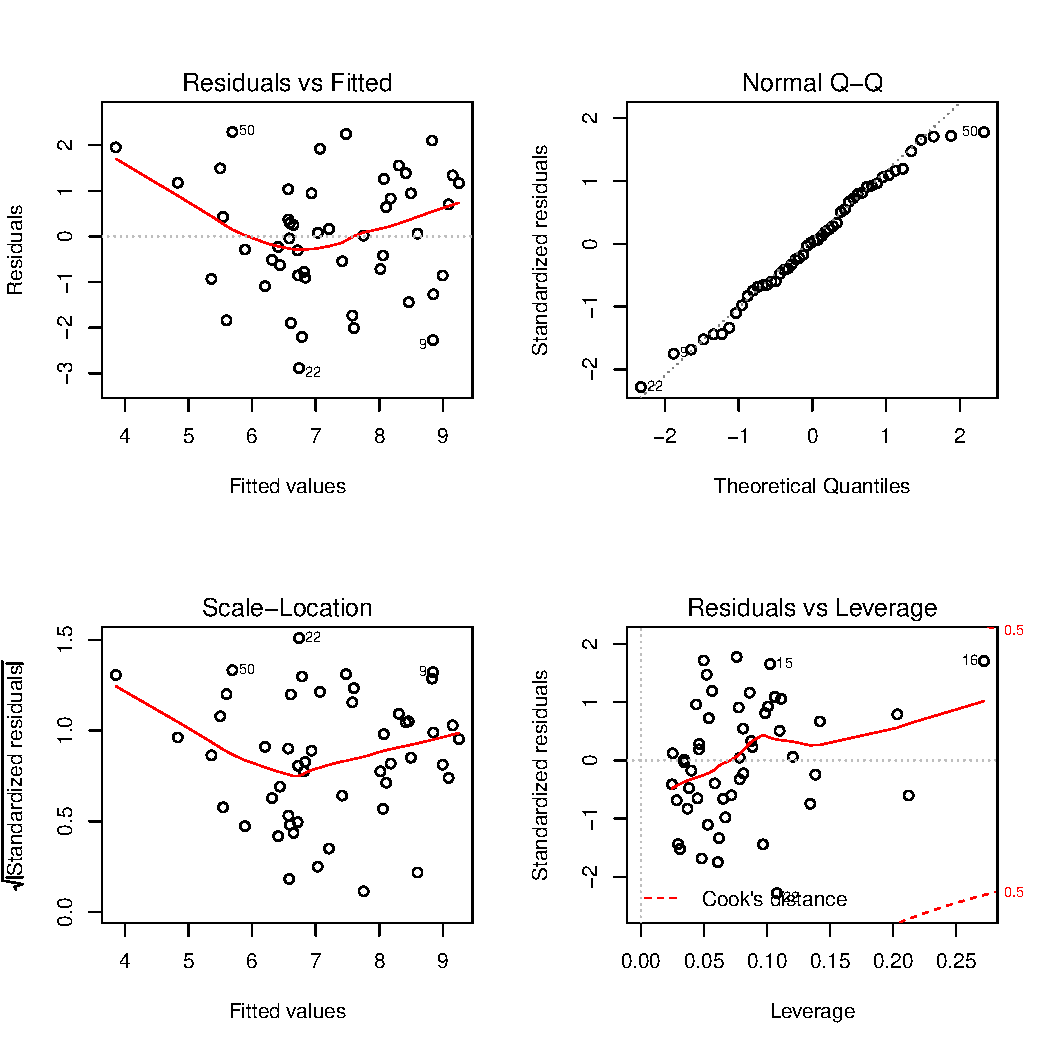
\includegraphics[width=.9\linewidth]{./figures/diag-lm.pdf}
\end{center}

The top left plot is useful to detect a misspecification of the linear
predictor (e.g. a U shape would indicate a missing quadratic
effect). The top right plot enable to check the normality of the
residuals, we will describe a more informative qqplot below. The
bottom left can be used to detect heteroschedasticity (e.g. a trumpet
shape) and the bottom right plot can be used to identify observation
that have a huge influence on the fitted values.

\subsubsection{Testing (A1)}
\label{sec:org0502a4f}

The qqtest package provides a more readable qqplot. To use it, we
first need to extract the residuals. This can be achieved using the
\texttt{residuals} method:
\lstset{language=r,label= ,caption= ,captionpos=b,numbers=none}
\begin{lstlisting}
dfW$resid.lm <- residuals(e.lm, type = "response")
\end{lstlisting}

The \texttt{type} argument indicates the type of residuals we want to
extract. Raw residuals are \(\hat{\varepsilon} = Y-\hat{Y}\), i.e. the
observed minus the fitted values. In models more complex than a
univariate linear regression, the raw residuals may not be iid. This
makes it difficult to assess the validity of the assumptions. In such
cases we display instead diagnostics for normalized residuals that, if
the assumptions of the model are correct, should follow a standard
normal distribution.

\bigskip

Having extracted the residuals, we can then obtain the qqplot using
the \texttt{qqtest} function:
\lstset{language=r,label= ,caption= ,captionpos=b,numbers=none}
\begin{lstlisting}
qqtest(dfW$resid.lm)
\end{lstlisting}

\begin{center}
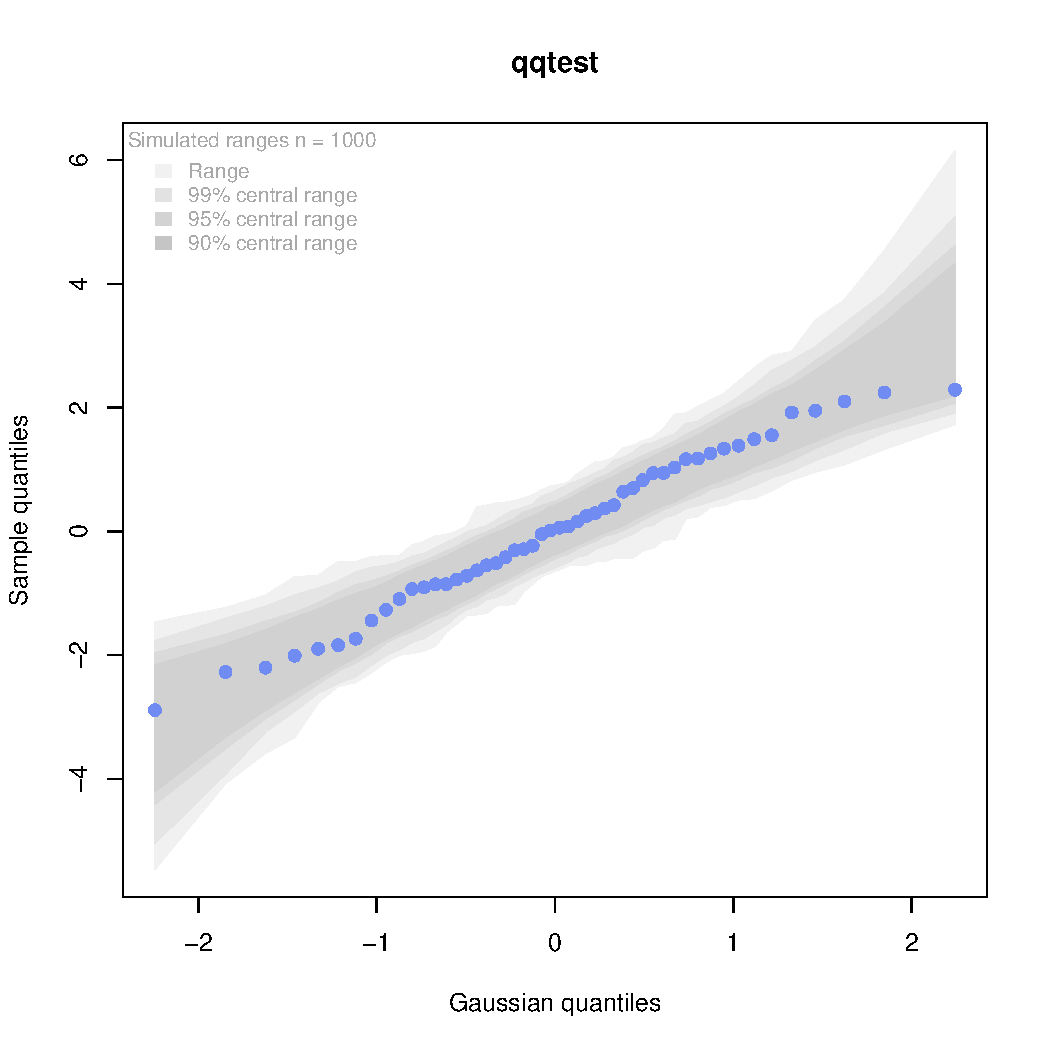
\includegraphics[width=.9\linewidth]{./figures/qqplot-lm.pdf}
\end{center}

The shaded area indicates where, if the normality assumption was
correct, we would expect to observe the points. Alternatively, an
histogram of the residuals can be used to assess the normality of the
residuals:
\lstset{language=r,label= ,caption= ,captionpos=b,numbers=none}
\begin{lstlisting}
hist(dfW$resid.lm, prob=TRUE, ylim = c(0,0.4))
curve(dnorm(x, mean=0, sd=1), add=TRUE, col = "red")
\end{lstlisting}

\begin{center}
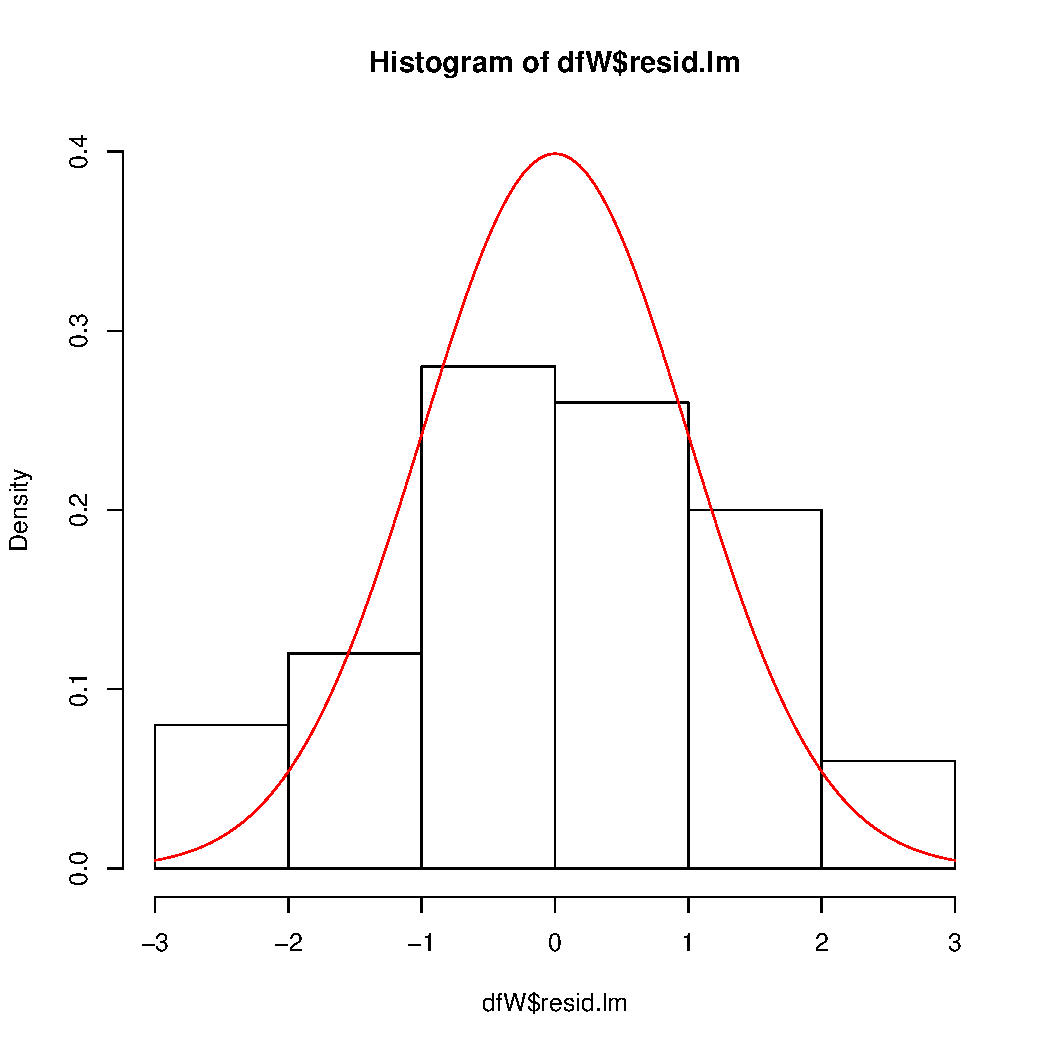
\includegraphics[width=.9\linewidth]{./figures/hist-lm.pdf}
\end{center}

Statistical tests can also be used to assess deviation from normality:
\lstset{language=r,label= ,caption= ,captionpos=b,numbers=none}
\begin{lstlisting}
shapiro.test(dfW$resid.lm)
\end{lstlisting}

\begin{verbatim}

	Shapiro-Wilk normality test

data:  dfW$resid.lm
W = 0.98104, p-value = 0.5967
\end{verbatim}
Here the null hypothesis is that the residuals follow a normal
distribution.

\clearpage

\subsubsection{Testing (A2)}
\label{sec:orga50855a}

A statistical test can also be used to assess whether there is
evidence for a more complex functional form for the linear predictor:
\lstset{language=r,label= ,caption= ,captionpos=b,numbers=none}
\begin{lstlisting}
cumres(e.lm)
\end{lstlisting}

\begin{verbatim}
Kolmogorov-Smirnov-test: p-value=0.195
Cramer von Mises-test: p-value=0.06
Based on 1000 realizations. Cumulated residuals ordered by predicted-variable.
---
Kolmogorov-Smirnov-test: p-value=0.016
Cramer von Mises-test: p-value=0.021
Based on 1000 realizations. Cumulated residuals ordered by age-variable.
---
Kolmogorov-Smirnov-test: p-value=0.151
Cramer von Mises-test: p-value=0.29
Based on 1000 realizations. Cumulated residuals ordered by BMI-variable.
---
Kolmogorov-Smirnov-test: p-value=0.708
Cramer von Mises-test: p-value=0.833
Based on 1000 realizations. Cumulated residuals ordered by MDI-variable.
---
\end{verbatim}

\subsubsection{Testing (A3)}
\label{sec:org00ff818}

The \texttt{influence} method can be used to output what is the impact of
each observation on each estimated parameter:
\lstset{language=r,label= ,caption= ,captionpos=b,numbers=none}
\begin{lstlisting}
head(influence(e.lm)$coefficient)
\end{lstlisting}

\begin{verbatim}
  (Intercept)           age           BMI           MDI
1 -0.06431419  0.0021223892  0.0011037299 -0.0023268582
2 -0.02333311  0.0005276379  0.0007260234 -0.0005075087
3  0.02225432 -0.0037807751  0.0134437130 -0.0084481492
4 -0.31091908  0.0087011324  0.0065717767 -0.0053971745
5 -0.16703438  0.0080674308 -0.0026717037 -0.0019605965
6  0.43406252  0.0002100576 -0.0176591598 -0.0008988258
\end{verbatim}

Large values (positive or negative) indicate influential observations.

\subsubsection{Testing (A4)}
\label{sec:org6e5096c}

The correlation among the explanatory variables can be assessed using
the VIF (variance inflation factor):
\lstset{language=r,label= ,caption= ,captionpos=b,numbers=none}
\begin{lstlisting}
car::vif(e.lm)
\end{lstlisting}

\begin{verbatim}
     age      BMI      MDI 
1.076066 1.034264 1.051645
\end{verbatim}
Values higher than 5 are considered as high (the threshold of 5 is
arbitrary).


\subsection{Hypothesis testing}
\label{sec:orgc9d99d6}

We want to formally test whether there is an effect of MDI on the
outcome. This is equivalent to test the null hypothesis:
\begin{align*}
(\Hypothesis[0]) \; \beta_{MDI,0} = 0
\end{align*}
 Since the parameters are estimated by ML and assuming that the model
is correctly specified, we know that the asymptotic distribution of
the parameter is Gaussian. This means that for large sample size, the
fluctuation of the estimated values follows a normal distribution. For
instance:
\begin{align*}
\hat{\beta} \underset{n \rightarrow \infty}{\sim} \Gaus[\beta,\sigma^2_\beta]
\end{align*}
where \(\sigma^2_\beta\) is the variance of the MLE, i.e. the
uncertainty surrounding our estimation of the association. It follows that:
\begin{align}
t_{\beta} = \frac{\hat{\beta}-\beta_0}{\sigma^2_\beta} \underset{n \rightarrow \infty}{\sim} \Gaus[0,1] \label{eq:uniWald}
\end{align}
So under the null hypothesis of no association between the outcome and
the exposure the statistic \(t_{\beta}\) should follow a standard
normal distribution. Very low or very large values are unlikely to be
observed and would indicate that the null hypothesis does not
hold. This is called a (univariate) Wald test. The result of this
tests can be obtained using the \texttt{summary} method \footnote{In reality R is automatically performing a correction that
improves the control of the type 1 error. Indeed we usually don't know
\(\sigma^2_\beta\) and plugging-in its estimate in equation
\eqref{eq:uniWald} modifies the distribution of \(t_{\beta}\) in small
samples. The correction uses a Student's t distribution instead of a
Gaussian distribution.}:
\lstset{language=r,label= ,caption= ,captionpos=b,numbers=none}
\begin{lstlisting}
summary(e.lm)$coef
\end{lstlisting}

\begin{verbatim}
                Estimate Std. Error    t value     Pr(>|t|)
(Intercept) -1.413215636 1.95732599 -0.7220134 4.739407e-01
age          0.006305252 0.03613264  0.1745030 8.622360e-01
BMI          0.247124506 0.05790521  4.2677422 9.756957e-05
MDI          0.151044284 0.03441289  4.3891775 6.598863e-05
\end{verbatim}

95\% confidence intervals for the model parameters can then be obtained
using the \texttt{confint} method:
\lstset{language=r,label= ,caption= ,captionpos=b,numbers=none}
\begin{lstlisting}
confint(e.lm)
\end{lstlisting}

\begin{verbatim}
                  2.5 %     97.5 %
(Intercept) -5.35310851 2.52667723
age         -0.06642598 0.07903648
BMI          0.13056736 0.36368165
MDI          0.08177473 0.22031384
\end{verbatim}

\clearpage

\section{Multivariate analysis using multiple univariate linear regressions}
\label{sec:multipleLM}
We now want to simultaneously test the effect of MDI on all the five
outcomes. To achieve it, we fit separately for each outcome a
univariate linear regression. Mathematically the model can be written:
\begin{align*}
\begin{bmatrix} 
Y_1  &= \alpha_{Y_{1}} + \beta_{Y_1,age} age + \beta_{Y_1,BMI} BMI + \beta_{Y_1,MDI} MDI + \varepsilon_{Y_1} \\
Y_2  &= \alpha_{Y_{2}} + \beta_{Y_2,age} age + \beta_{Y_2,BMI} BMI + \beta_{Y_2,MDI} MDI + \varepsilon_{Y_2} \\
Y_3  &= \alpha_{Y_{3}} + \beta_{Y_3,age} age + \beta_{Y_3,BMI} BMI + \beta_{Y_3,MDI} MDI + \varepsilon_{Y_3} \\
Y_4  &= \alpha_{Y_{4}} + \beta_{Y_4,age} age + \beta_{Y_4,BMI} BMI + \beta_{Y_4,MDI} MDI + \varepsilon_{Y_4} \\
Y_5  &= \alpha_{Y_{5}} + \beta_{Y_5,age} age + \beta_{Y_5,BMI} BMI + \beta_{Y_5,MDI} MDI + \varepsilon_{Y_5} 
\end{bmatrix} 
\end{align*}
where
\(\varepsilon_{1},\varepsilon_{2},\varepsilon_{3},\varepsilon_{4},\varepsilon_{5}\)
are the residual errors. The residuals are assumed to have zero mean
and finite variance, respectively,
\(\sigma^2_{1},\sigma^2_{2},\sigma^2_{3},\sigma^2_{4},\sigma^2_{5}\). Here
we make no assumption on the correlation structure between the
residuals.

\subsection{Fitting multiple linear regression in \Rlogo{}}
\label{sec:orgd3260cb}

We can estimate all the 5 models and store them into a list:
\lstset{language=r,label= ,caption= ,captionpos=b,numbers=none}
\begin{lstlisting}
ls.lm <- list(Y1 = lm(Y1 ~ age + BMI + MDI, data = dfW),
			  Y2 = lm(Y2 ~ age + BMI + MDI, data = dfW),
			  Y3 = lm(Y3 ~ age + BMI + MDI, data = dfW),
			  Y4 = lm(Y4 ~ age + BMI + MDI, data = dfW),
			  Y5 = lm(Y5 ~ age + BMI + MDI, data = dfW)
			  )
\end{lstlisting}

\subsection{Interpretation of the regression coefficients}
\label{sec:orga3cb513}

Same as in the univariate case (see section \ref{sec:interpretationLM}).

\subsection{Diagnostics tools for univariate linear regression in \Rlogo{}}
\label{sec:org7cc3cb1}

Same as in the univariate case (see section \ref{sec:diagLM}). This model
checking needs to be done for each outcome.

\subsection{Hypothesis testing}
\label{sec:org038e05b}

We now want to test:
\begin{align*}
(\Hypothesis[0]) \; \beta_{Y_1, MDI, 0} = 0
 \text{ and } \beta_{Y_2, MDI, 0} = 0
 \text{ and } \beta_{Y_3, MDI, 0} = 0
 \text{ and } \beta_{Y_4, MDI, 0} = 0
 \text{ and } \beta_{Y_5, MDI, 0} = 0
\end{align*}

The p-values returned by \texttt{summary} are no more valid since we are
performing multiple tests (here 5 tests). A basic solution would be to
collect the p-values:
\lstset{language=r,label= ,caption= ,captionpos=b,numbers=none}
\begin{lstlisting}
vec.p.value <- unlist(lapply(ls.lm, function(x){
	summary(x)$coef["MDI","Pr(>|t|)"]
}))
\end{lstlisting}

\clearpage

and adjust them for multiple comparisons using Bonferroni:
\lstset{language=r,label= ,caption= ,captionpos=b,numbers=none}
\begin{lstlisting}
p.adjust(vec.p.value, method = "bonferroni")
\end{lstlisting}

\begin{verbatim}
          Y1           Y2           Y3           Y4           Y5 
3.299432e-04 4.218369e-02 3.552579e-01 2.276690e-07 8.565878e-01
\end{verbatim}

While easy to use this approach tends to be too conservative
(i.e. give to large p-values) when the test statistics are
correlated. This is usually the case when the outcomes are
correlated. We will therefore use a more efficient correction called
the Dunnett approach. First we need to define the null hypothesis
that we want to test via a contrast matrix. For simple null hypotheses
like the one we are considering in this example, we can use the
function \texttt{createContrast} that will create the matrix for us:
\lstset{language=r,label= ,caption= ,captionpos=b,numbers=none}
\begin{lstlisting}
resC <- createContrast(ls.lm, var.test = "MDI", add.variance = TRUE)
\end{lstlisting}

This function defines for each model the appropriate contrast matrix:
\lstset{language=r,label= ,caption= ,captionpos=b,numbers=none}
\begin{lstlisting}
resC$mlf
\end{lstlisting}
\begin{verbatim}
$Y1
    (Intercept) age BMI MDI sigma2
MDI           0   0   0   1      0

$Y2
    (Intercept) age BMI MDI sigma2
MDI           0   0   0   1      0

$Y3
    (Intercept) age BMI MDI sigma2
MDI           0   0   0   1      0

$Y4
    (Intercept) age BMI MDI sigma2
MDI           0   0   0   1      0

$Y5
    (Intercept) age BMI MDI sigma2
MDI           0   0   0   1      0

attr(,"class")
[1] "mlf"
\end{verbatim}

and right hand side of the null hypothesis:
\lstset{language=r,label= ,caption= ,captionpos=b,numbers=none}
\begin{lstlisting}
resC$null
\end{lstlisting}

\begin{verbatim}
Y1: MDI Y2: MDI Y3: MDI Y4: MDI Y5: MDI 
      0       0       0       0       0
\end{verbatim}

\clearpage

We will now call \texttt{glht2} to perform the adjustment for multiple
comparisons but first we need to convert the list into a \texttt{mmm} object:
\lstset{language=r,label= ,caption= ,captionpos=b,numbers=none}
\begin{lstlisting}
class(ls.lm) <- "mmm"
e.glht_lm <- glht2(ls.lm, linfct = resC$contrast, rhs = resC$null)
e.glht_lm
\end{lstlisting}

\begin{verbatim}
	 General Linear Hypotheses

Linear Hypotheses:
             Estimate
Y1: MDI == 0  0.15104
Y2: MDI == 0  0.16770
Y3: MDI == 0  0.14907
Y4: MDI == 0  0.19860
Y5: MDI == 0  0.09806
\end{verbatim}

We can now correct for multiple comparisons using the (single-step)
Dunnett approach:
\lstset{language=r,label= ,caption= ,captionpos=b,numbers=none}
\begin{lstlisting}
summary(e.glht_lm, test = adjusted("single-step"))
\end{lstlisting}

\begin{verbatim}
	 Simultaneous Tests for General Linear Hypotheses

Linear Hypotheses:
             Estimate Std. Error t value Pr(>|t|)    
Y1: MDI == 0  0.15104    0.03441   4.389   <0.001 ***
Y2: MDI == 0  0.16770    0.06093   2.752   0.0286 *  
Y3: MDI == 0  0.14907    0.08067   1.848   0.1996    
Y4: MDI == 0  0.19860    0.03039   6.535   <0.001 ***
Y5: MDI == 0  0.09806    0.07057   1.390   0.4208    
---
Signif. codes:  0 '***' 0.001 '**' 0.01 '*' 0.05 '.' 0.1 ' ' 1
(Adjusted p values reported -- single-step method)
\end{verbatim}

Note that the p-value for the global test equals to the smallest
 p-value. This means that we reject the global null hypothesis
 whenever we reject the null hypothesis for any of the outcome (after
 adjustment for multiple comparisons!).


For comparison one can change the argument in \texttt{adjust} to apply the
Bonferroni adjustment:
\lstset{language=r,label= ,caption= ,captionpos=b,numbers=none}
\begin{lstlisting}
summary(e.glht_lm, test = adjusted("bonferroni"))
\end{lstlisting}

\begin{verbatim}
	 Simultaneous Tests for General Linear Hypotheses

Linear Hypotheses:
             Estimate Std. Error t value Pr(>|t|)    
Y1: MDI == 0  0.15104    0.03441   4.389  0.00033 ***
Y2: MDI == 0  0.16770    0.06093   2.752  0.04218 *  
Y3: MDI == 0  0.14907    0.08067   1.848  0.35526    
Y4: MDI == 0  0.19860    0.03039   6.535 2.28e-07 ***
Y5: MDI == 0  0.09806    0.07057   1.390  0.85659    
---
Signif. codes:  0 '***' 0.001 '**' 0.01 '*' 0.05 '.' 0.1 ' ' 1
(Adjusted p values reported -- bonferroni method)
\end{verbatim}

Finally, confidence intervals can be obtained using the \texttt{confint}
function:
\lstset{language=r,label= ,caption= ,captionpos=b,numbers=none}
\begin{lstlisting}
confint(e.glht_lm)
\end{lstlisting}

\begin{verbatim}
	 Simultaneous Confidence Intervals

Fit: NULL

Quantile = 2.5215
95% family-wise confidence level
 

Linear Hypotheses:
             Estimate lwr      upr     
Y1: MDI == 0  0.15104  0.06427  0.23782
Y2: MDI == 0  0.16770  0.01407  0.32133
Y3: MDI == 0  0.14907 -0.05434  0.35248
Y4: MDI == 0  0.19860  0.12197  0.27524
Y5: MDI == 0  0.09806 -0.07987  0.27599
\end{verbatim}
Note that by default the \texttt{confint} function output confidence
intervals using the (single-step) Dunnett approach.


\clearpage

\section{References}
\label{sec:org6a582b5}

\begingroup
\renewcommand{\section}[2]{}
\bibliographystyle{apalike}
\bibliography{bibliography} 
\endgroup

\clearpage

\appendix

\section{Statistics: definitions and notations}
\label{SM:statistics}
\subsection{Variables}
\label{sec:orge3bd53a}

We can differentiate several types of random variables: outcomes,
exposure, risk factors, confounders, and mediators. To explicit the
difference between these types of variables we consider a set of
random variables \((Y,E,X_1,X_2,M)\) whose relationships are
displayed on \autoref{fig:pathDiagram}:
\begin{itemize}
\item \textbf{outcome} (\(Y\)): random variables that are observed with noise. It
can be for instance the 5HT-4 binding in a specific brain
region. When considering several outcomes we will denote in bold
variable that stands for a vector of random variables:
\(\mathbf{Y}=(Y_1,Y_2,\ldots,Y_m)\). This happens for instance when
studying the binding in several brain regions. In such a case we
expect the outcomes to be correlated.
\item \textbf{exposure} (\(E\)): a variable that may affect the outcome or be
associated with the outcome \emph{and} we are interested in studying this
effect/association. It can for instance be a genetic factor that is
hypothesized to increase the 5HT-4 binding, or a disease like
depression that is associated with a change in binding (we don't
know whether one causes the other or whether they have a common
cause, e.g. a genetic variant).
\item \textbf{risk factor/confounder} (\(X_1,X_2\)): a variable that
may affect the outcome or be associated with the outcomes \emph{but} we
are \emph{not} interested in studying their effect/association. Risk
factors (denoted by \(X_1\)) are only associated with the outcomes
and confounders that are both associated with the outcome and the
exposure. We usually need to account for confounders the statistical
model in order to obtain unbiased estimates while accounting for
risk factors only enables to obtain more precise estimates (at least
in linear models).
\item \textbf{mediator} (\(M\)): a variable that modulate the effect of the
exposure, i.e. stands on the causal pathway between the exposure and
the outcome. For instance, the permeability of the blood-brain
barrier may modulate the response to drugs and can act as a
mediator. It is important to keep in mind that when we are
interested in the (total) effect of \(E\) on \(Y\), we should \emph{not}
adjust the analysis on \(M\)\footnote{This may not be true in specific types of confounding but we
will ignore that.}. Doing so we would remove the effect of
\(E\) mediated by \(M\) and therefore bias the estimate of the total
effect (we would only get the direct effect).
\end{itemize}

In the following we will assume that we do not measure any mediator
variable and therefore ignore this type of variable. Also we will call
\textbf{covariates} the variables \(E,X_1,X_2\).

\begin{figure}[htbp]
\centering
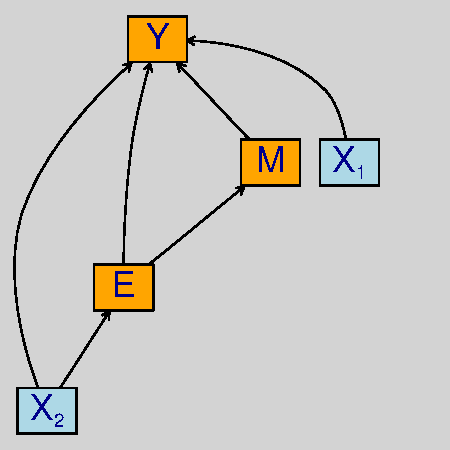
\includegraphics[width=0.7\textwidth]{./figures/pathDiagram.pdf}
\caption{\label{fig:pathDiagram}
Path diagram relating the variables Y, E, M, \(X_1\) and \(X_2\)}
\end{figure}

\clearpage 

\subsection{Assumptions}
\label{sec:orgb182bdb}

We can distinguish two types of assumptions:
\begin{itemize}
\item \textbf{causal assumptions}: saying which variables are related and in
which direction. This can be done by drawing a path diagram similar
to \autoref{fig:pathDiagram}. In simple univariate models it may seems
unnecessary to draw the path diagram since the system of variables is
very simple to visualize. In multivariate model, it is often very
useful to draw it. Some of these assumptions are untestable,
e.g. often we cannot decide whether it is \(E\) that impacts \(Y\)
or whether it is \(Y\) that impacts \(E\) just based on the data.

\item \textbf{modeling assumptions}: specifying the type of relationship between
variables (e.g. linear) and the marginal or joint distribution
(e.g. Gaussian). Often these assumptions can be tested and relaxed
using a more flexible model. While appealing, there are some
drawbacks with using a very flexible model: more data are needed to
get precise estimates and the interpretation of the results is more
complex.
\end{itemize}

\subsection{Statistical model}
\label{sec:org532bc2a}
A statistical model \(\model\) is set of possible probability
distributions. For instance when we fit a Gaussian linear model for
\(Y_1\) with just an intercept \(\model=\left\{\Gaus[\mu,\sigma^2];\mu
\in \Real, \; \sigma^2 \in \Real^+ \right\}\): \(\model\) is the set
containing all possible univariate normal distributions.

\subsection{Model parameters}
\label{sec:orgf69b02d}

The model parameters are the (non random) variables that enable the
statistical model to "adapt" to different settings. They will be
denoted \(\Theta\). They are the one that are estimated when we fit
the statistical model using the data or that we specify when we
simulate data. In the previous example, we could simulate data
corresponding to a Gaussian linear model using the \texttt{rnorm} function in
R:
\lstset{language=r,label= ,caption= ,captionpos=b,numbers=none}
\begin{lstlisting}
rnorm
\end{lstlisting}

\begin{verbatim}
function (n, mean = 0, sd = 1) 
.Call(C_rnorm, n, mean, sd)
<bytecode: 0x000000001d7eb938>
<environment: namespace:stats>
\end{verbatim}

We would need to specify:
\begin{itemize}
\item \(n\) the sample size
\item \(\Theta=(\mu,\sigma^2)\) the model parameters, here \(\mu\) corresponds to \texttt{mean} and \(\sigma\) to \texttt{sd}.
\end{itemize}

\bigskip

The true model parameters are the model parameters that have generated
the observed data. They will be denoted \(\Theta_0\). For instance if
in reality the binding potential is normally distributed with mean 5
and variance \(2^2=4\), then
\(\Theta_0=(\mu_0,\sigma_0^2)=(5,4)\). Then doing our experiment we
observed data such as:
\lstset{language=r,label= ,caption= ,captionpos=b,numbers=none}
\begin{lstlisting}
set.seed(10)
Y_1.XP1 <- rnorm(10, mean = 5, sd = 2)
Y_1.XP1
\end{lstlisting}

\begin{verbatim}
[1] 5.037492 4.631495 2.257339 3.801665 5.589090 5.779589 2.583848 4.272648 1.746655 4.487043
\end{verbatim}

If we were to re-do the experiment we would observe new data but \(\Theta_0\) would not change:
\lstset{language=r,label= ,caption= ,captionpos=b,numbers=none}
\begin{lstlisting}
Y_1.XP2 <- rnorm(10, mean = 5, sd = 2)
Y_1.XP2
\end{lstlisting}

\begin{verbatim}
[1] 7.203559 6.511563 4.523533 6.974889 6.482780 5.178695 3.090112 4.609699 6.851043 5.965957
\end{verbatim}

The estimated parameters are the parameters that we estimate when we
fit the statistical model. They will be denoted \(\hat{\Theta}\). We
usually try to find parameters whose value maximize the chance of
simulating the observed data under the estimated model (maximum
likelihood estimation, MLE). For instance in the first experiment all
values are positive so we would not estimate a negative mean value. In
our example, \(\hat{\mu}\) the MLE of \(\mu\) reduces to the empirical
average and \(\hat{\sigma}^2\) the MLE of \(\sigma^2\) to the
empirical variance:
\lstset{language=r,label= ,caption= ,captionpos=b,numbers=none}
\begin{lstlisting}
Theta_hat.XP1 <- c(mu_hat = mean(Y_1.XP1),
				   sigma2_hat = var(Y_1.XP1))
Theta_hat.XP1
\end{lstlisting}

\begin{verbatim}
  mu_hat sigma2_hat 
4.018686   1.959404
\end{verbatim}

Clearly the estimated coefficients vary across experiments:
\lstset{language=r,label= ,caption= ,captionpos=b,numbers=none}
\begin{lstlisting}
Theta_hat.XP2 <- c(mu_hat = mean(Y_1.XP2),
				   sigma2_hat = var(Y_1.XP2))
Theta_hat.XP2
\end{lstlisting}

\begin{verbatim}
  mu_hat sigma2_hat 
5.739183   1.799311
\end{verbatim}

\subsection{Parameter of interest}
\label{sec:org3782e89}

The statistical model may contain many parameters, most of them are
often not of interest but are needed to obtain valid estimates
(e.g. account for confounders). In most settings, the parameter of
interest is one (or several) model parameter(s) - or simple
transformation of them. For instance if we are interested in the
average binding potential in the population our parameter of interest
is \(\mu\).

\bigskip

Often, the aim of a study is to obtain the best estimate of the
parameter of interest \(\mu\). Best means:
\begin{itemize}
\item \textbf{unbiased}: if we were able to replicate the study many times,
i.e. get several estimates \(\hat{\mu}_1,\hat{\mu}_2,\ldots,\hat{\mu}_K\), the
average estimate \(<\hat{\mu}>=\frac{\hat{\mu}_1+\hat{\mu}_2+\ldots+\hat{\mu}_K}{K}\) would coincide with the true one \(\mu_0\).
\item \textbf{minimal variance}: if we were able to replicate the study many
times, the variance of the estimates
\(\frac{(\hat{\mu}_1-<\hat{\mu}>)^2+\ldots+(\hat{\mu}_K-<\hat{\mu}>)^2}{K-1}\)
should be as low as possible.
\end{itemize}

There will often be a trade-off between these two objectives. A very
flexible method is more likely to give an unbiased estimate
(e.g. being able to model non-linear relationship) at the price of
greater uncertainty about the estimates. Often we favor unbiasedness
over minimal variance. Indeed, if several studies are published with
the same parameter of interest, one can pool the results to obtain an
estimate with lower variance. Note that we have no guarantee that it
will reduce the bias.

\subsection{Contrast matrix}
\label{sec:org4346371}

When dealing with many parameters it is convenient to define the null
hypothesis via a contrast matrix. An example of null hypothesis is:
\begin{align*}
(\Hypothesis[0]) \; \beta_{MDI,0} = 0
\end{align*}
If we consider \(\Theta=(\alpha,\beta_{age},\beta_{BMI},\beta_{MDI})\),
this null hypothesis can be equivalently written:

\begin{align*}
c=[0 \; 0 \; 0 \; 1]
\end{align*}
such that: 
\begin{align*}
(\Hypothesis[0]) \; c \trans{\Theta}_{0} = 0
\end{align*}
Indeed
\begin{align*}
c \trans{\Theta}_{0} = 0 * \alpha_0 + 0 * \beta_{age,0} + 0 * \beta_{BMI,0} + 1 * \beta_{MDI,0} = \beta_{MDI,0}
\end{align*}

An example where the contrast matrix is useful is
\begin{itemize}
\item when one wish to test linear combination of parameters,
e.g. consider the null hypothesis:
\end{itemize}
\begin{align*}
(\Hypothesis[0]) \; \beta_{MDI,0} = \beta_{BMI,0}
\end{align*}
Here the contrast matrix would be:
\begin{align*}
c=[0 \; 0 \; -1 \; 1]
\end{align*}
\begin{itemize}
\item when one wish to test several hypotheses simultaneously,
e.g. consider the null hypothesis:
\end{itemize}
\begin{align*}
(\Hypothesis[0]) \; \beta_{BMI,0} = 0 \text{ or } \beta_{MDI,0} = 0 \\
\end{align*}
Here the contrast matrix would be:
\begin{align*}
C = \begin{bmatrix}
0 & 0 & 1 & 0 \\
0 & 0 & 0 & 1 \\
\end{bmatrix}
\end{align*}

In \Rlogo{}, the method \texttt{createContrast} helps to define the contrast
matrix:
\lstset{language=r,label= ,caption= ,captionpos=b,numbers=none}
\begin{lstlisting}
Clin <- createContrast(e.lm, par = c("MDI - BMI = 0"),
					   add.variance = FALSE, rowname.rhs = FALSE)
Clin$contrast
\end{lstlisting}

\begin{verbatim}
            (Intercept) age BMI MDI
- BMI + MDI           0   0  -1   1
\end{verbatim}

\lstset{language=r,label= ,caption= ,captionpos=b,numbers=none}
\begin{lstlisting}
Csim <- createContrast(e.lm, par = c("BMI = 0","MDI = 0"),
					   add.variance = FALSE, rowname.rhs = FALSE)
Csim$contrast
\end{lstlisting}

\begin{verbatim}
    (Intercept) age BMI MDI
BMI           0   0   1   0
MDI           0   0   0   1
\end{verbatim}

Then the contrast matrix can be send to \texttt{glht} to obtain p-values and
confidence intervals:
\lstset{language=r,label= ,caption= ,captionpos=b,numbers=none}
\begin{lstlisting}
elin.glht <- glht(e.lm, linfct = Clin$contrast)
summary(elin.glht)
\end{lstlisting}

\begin{verbatim}

	 Simultaneous Tests for General Linear Hypotheses

Fit: lm(formula = Y1 ~ age + BMI + MDI, data = dfW)

Linear Hypotheses:
                 Estimate Std. Error t value Pr(>|t|)
- BMI + MDI == 0 -0.09608    0.06993  -1.374    0.176
(Adjusted p values reported -- single-step method)
\end{verbatim}

\lstset{language=r,label= ,caption= ,captionpos=b,numbers=none}
\begin{lstlisting}
esim.glht <- glht(e.lm, linfct = Csim$contrast)
summary(esim.glht)
\end{lstlisting}

\begin{verbatim}
	 Simultaneous Tests for General Linear Hypotheses

Fit: lm(formula = Y1 ~ age + BMI + MDI, data = dfW)

Linear Hypotheses:
         Estimate Std. Error t value Pr(>|t|)    
BMI == 0  0.24712    0.05791   4.268 0.000195 ***
MDI == 0  0.15104    0.03441   4.389 0.000132 ***
---
Signif. codes:  0 '***' 0.001 '**' 0.01 '*' 0.05 '.' 0.1 ' ' 1
(Adjusted p values reported -- single-step method)
\end{verbatim}
\end{document}